\chapter{Implementierung des Frameworks zur simulationsbasierten
Validierung}
\label{sec:framework}
Kern der Arbeit ist die Entwicklung eines Frameworks zur Detektion von Fehlern
bei der Ausführung von Roboterprogrammcode. In diesem Kapitel werden
die technischen Grundlagen sowie das Vorgehen zur
Implementierung des Frameworks so beschrieben und anschließend ein Testszenario
entwickelt, welches zur Validierung des entwickelten Frameworks dienen soll.

\section{Architektur des Frameworks}
\label{sec:architektur_frameowork}
Das entwickelte Framework ist in Unity implementiert und basiert auf einem digitalen
Zwilling des Roboters, der die Zustände der einzelnen Achsen und relevanten
Systemkomponenten kontinuierlich bereitstellt. Darauf aufbauend sind die
Überwachungsmodule (\textit{Monitore}) integriert, die unterschiedliche
Aspekte des Roboterverhaltens beobachten und als Safety Events dokumentieren.


Im Folgenden wird erläutert, wie das Framework funktional, architektonisch und
algorithmisch implemeniert ist. Wichtig dabei sind dabei folgende Annahmen zu
beachten, die sich in Kapitel \ref{sec:aufbauTestszenario} wiederfinden: Als
Testobjekt wird ein ABB IRB 6700-235/2.65 Roboter verwendet. Dabei handelt es
sich um einen Knickarmroboter mit 6 Freiheitsgraden und 6
Gelenken.\vglcite{abbirb2025} Dieser wird in RobotStudio Version 2025.3
simuliert und mittels eines OmniCore-Controllers gesteuert.

\subsection{Funktionale Anforderungen}

Die funktionalen Anforderungen an das Framework
lassen sich in zwei Hauptkategorien unterteilen: die \textbf{Echtzeitüberwachung
	kritischer Roboterzustände} und Programmablaufereignisse sowie die \textbf{systematische
	Protokollierung} der auftretenden Ereignisse.

\subsubsection{Überwachungsfunktionen}

Das Framework muss vier zentrale Überwachungsfunktionen implementieren:

\begin{enumerate}
	\item \textbf{Kollisionserkennung}: Identifikation von Kontakten zwischen Roboterkomponenten und Objekten in der Arbeitsumgebung sowie Selbstkollisionen zwischen benachbarten Gliedern der kinematischen Kette.

	\item \textbf{Singularitätserkennung}: Frühzeitige Erkennung kinematischer Singularitäten (Handgelenk-, Schulter- und Ellbogensingularitäten), die zu Kontrollverlust oder undefinierten Bewegungen führen können.

	\item \textbf{Prozessflussüberwachung}: Validierung der korrekten Abfolge von Bearbeitungsstationen für Werkstücke und Erkennung von Abweichungen von der spezifizierten Sequenz.

	\item \textbf{Gelenkdynamiküberwachung}: Kontinuierliche Überprüfung von Gelenkwinkeln, -geschwindigkeiten und -beschleunigungen auf Grenzwertüberschreitungen, insbesondere während der Handhabung von Werkstücken.
\end{enumerate}

\subsubsection{Systematische Ereignisprotokollierung}

Mithilfe des Frameworks soll es möglichh sein, die genannten Fehlerarten
systematisch debuggen zu können und die Fehlersuche in Roboterprogrammcode zu
vereinfachen. Neben der reinen Erkennung ist die folglich eine formalisierte
Dokumentation der Ereignisse notwendig. Jedes detektierte Ereignis soll mit
entsprechenden Metadaten zum aktuellen Status des Roboters angereicht werden.
Folgende Metadaten lassen sich nach initialem Testen mithilfe der zur Verfügung
stehenden Tools extrahieren:

\begin{itemize}
	\item \textbf{Zeitlicher Kontext}: Präziser Zeitstempel des Ereignisses mit Millisekunden-Auflösung
	\item \textbf{Räumlicher Kontext}: Vollständige Gelenkwinkelkonfiguration und TCP-Position zum Ereigniszeitpunkt
	\item \textbf{Programmkontext}: Aktuelles Modul, Routine und Programmzeile der Robotersteuerung
	\item \textbf{Ereignisspezifische Daten}: Je nach Ereignistyp relevante Zusatzinformationen (Kollisionspunkt, Singularitätstyp, Sequenzabweichung, Grenzwertüberschreitung)
\end{itemize}
\noindent
Diese strukturierte Erfassung ermöglicht die nachgelagerte genaue Auswertung der
vorhandenen Daten und soll das Debuggen des Programmcodes und das Erkennen von
Schwachstellen erleichtern.

\subsection{Zielsetzung und architektonische Anforderungen}
Der Stand der Technik aktueller Simulationsplattformen für Roboter zeigt, dass
virtuelle Steuerungen und damit zusammenhängende Simulationsplattformen
herstellerspezifisch entwickelt und mit Ausnahme von ROS keine einheitliche
Schnittstelle zur Kommunikation mit externen Plattformen oder Physik-Engines
bieten. Somit muss für jeden Robotertyp ein designierter Konnektor genutzt
werden, um diesen mit einer externen, herstellerunabhängigen Simulationplattform
zu verbinden. Um eine herstellerunabhängige und erweiterbare Plattform zu
entwickeln, sollte also eine gemeinsame Schnittstelle implementiert werden.\\

\noindent
Zusammenfassend verfolgt die Architektur des Frameworks drei zentrale Ziele:
\begin{enumerate}
	\item \textbf{Vendor-Agnostik}: Abstraktion verschiedener Roboterhersteller durch einheitliche Interface-basierte Architektur ohne herstellerspezifische Abhängigkeiten im Kern-Framework

	\item \textbf{Modulare Erweiterbarkeit}: Plugin-System für Safety Monitoring Module und Kommunikationsprotokolle ohne Änderungen der bestehenden Architektur

	\item \textbf{Echtzeitfähige Kommunikation}: Latenzarme Datenübertragung für Motion Control und ereignisbasierte Sicherheitsüberwachung
\end{enumerate}

\subsection{Unity3D als Simulationsplattform}

Die Wahl von Unity3D als zugrundeliegende Simulationsplattform basiert auf
mehreren technischen und praktischen Erwägungen. Während es bereits mehrere
kommerzielle Programme für die Gestaltung und Simulation von Robotern in
virtuellen Umgebungen gibt, sind diese nur selten mit anderen CAD-Systemen und
Robotern kompatibel, unterstützen nicht alle Roboterbibliotheken oder werden
nur plattformabhängig angeboten (vgl. \vglcite[247]{andaluz2016}). Unity3D
hingegen ist mit den meisten CAD-Systemen kompatibel und bietet eine
plattformübergreifende Lösung.\\

\noindent
Unity3D bietet eine ausgereifte 3D-Rendering-Pipeline mit integrierter
Physik-Engine, welche zur Simulation von Gegenständen mit realitätsnahem
Verhalten sowie komplexen Arbeitsräumen geeignet ist \vglcites{\cite@single{Unity2025SystemRequirements};\cite@single{Unity2025PhysicsOverview}}.
Die Engine wurde bereits erfolgreich in der wissenschaftlichen Forschung
eingesetzt und bietet Module und Plugins für spezifische Anwendungsfälle im
Simulationsbereich. Unity3D ermöglicht es auch Nicht-Programmierern,
leistungsstarke Animations- und Interaktionsdesign-Tools zu nutzen, um Roboter
visuell zu programmieren und zu animieren.\vglcite[431]{bartneck2015}\\

\noindent
Technisch ermöglicht Unity3D durch seine Scripting-Runtime (basierend auf
Mono/.NET Framework) die Verwendung moderner C\#-Sprachfeatures für
nebenläufige Prozesse und asynchroner Programmierung
\vglcite{unity_async_2023}, was es ermöglicht, Visualisierung,
Datenakquise und Überwachung zu trennen. Die .NET-basierte Architektur
unterstützt dabei sowohl Task-basierte asynchrone Operationen als auch
Coroutines für zeitgesteuerte Prozesse
\vglcite{unity_coroutines_2023}, welche die notwendige periodische
Ausführung von Prozessen auf verschiedenen Ebenen des Frameworks stark
vereinfacht.\\

\noindent
in weiterer Vorteil für die Robotik-Simulation liegt in der
Verfügbarkeit visueller Programmiertools und der integrierten
Entwicklungsumgebung. Die Plattform bietet umfangreiche Debugging- und
Profiling-Werkzeuge (Unity Profiler, Frame Debugger), die während der
Entwicklung und zur Laufzeit genutzt werden können
\vglcite{unity_profiler_2023}. Diese Werkzeuge ermöglichen die
Analyse von Performance-Engpässen bei der Verarbeitung von Roboterdaten und die
Optimierung der Sicherheitsmonitor-Updates.

Darüber hinaus lassen sich während der Laufzeit sowohl die Szene (hier: die
Roboterzelle) als auch Komponenten-Parameter in Echtzeit bearbeiten und
einsehen \vglcite[1236]{haas2022}, was das Debuggen und Testen
beschleunigt.


\subsection{Systemarchitektur}

Das entwickelte Framework implementiert eine vierschichtige Architektur, die
eine klare Trennung der Verantwortlichkeiten gewährleistet (siehe Abbildung
\ref{fig:layer_architecture}). Diese Strukturierung folgt etablierten
Software-Engineering-Prinzipien, um Wartbarkeit und Erweiterbarkeit zu
gewährleisten.

\begin{figure}[H]
	\centering
	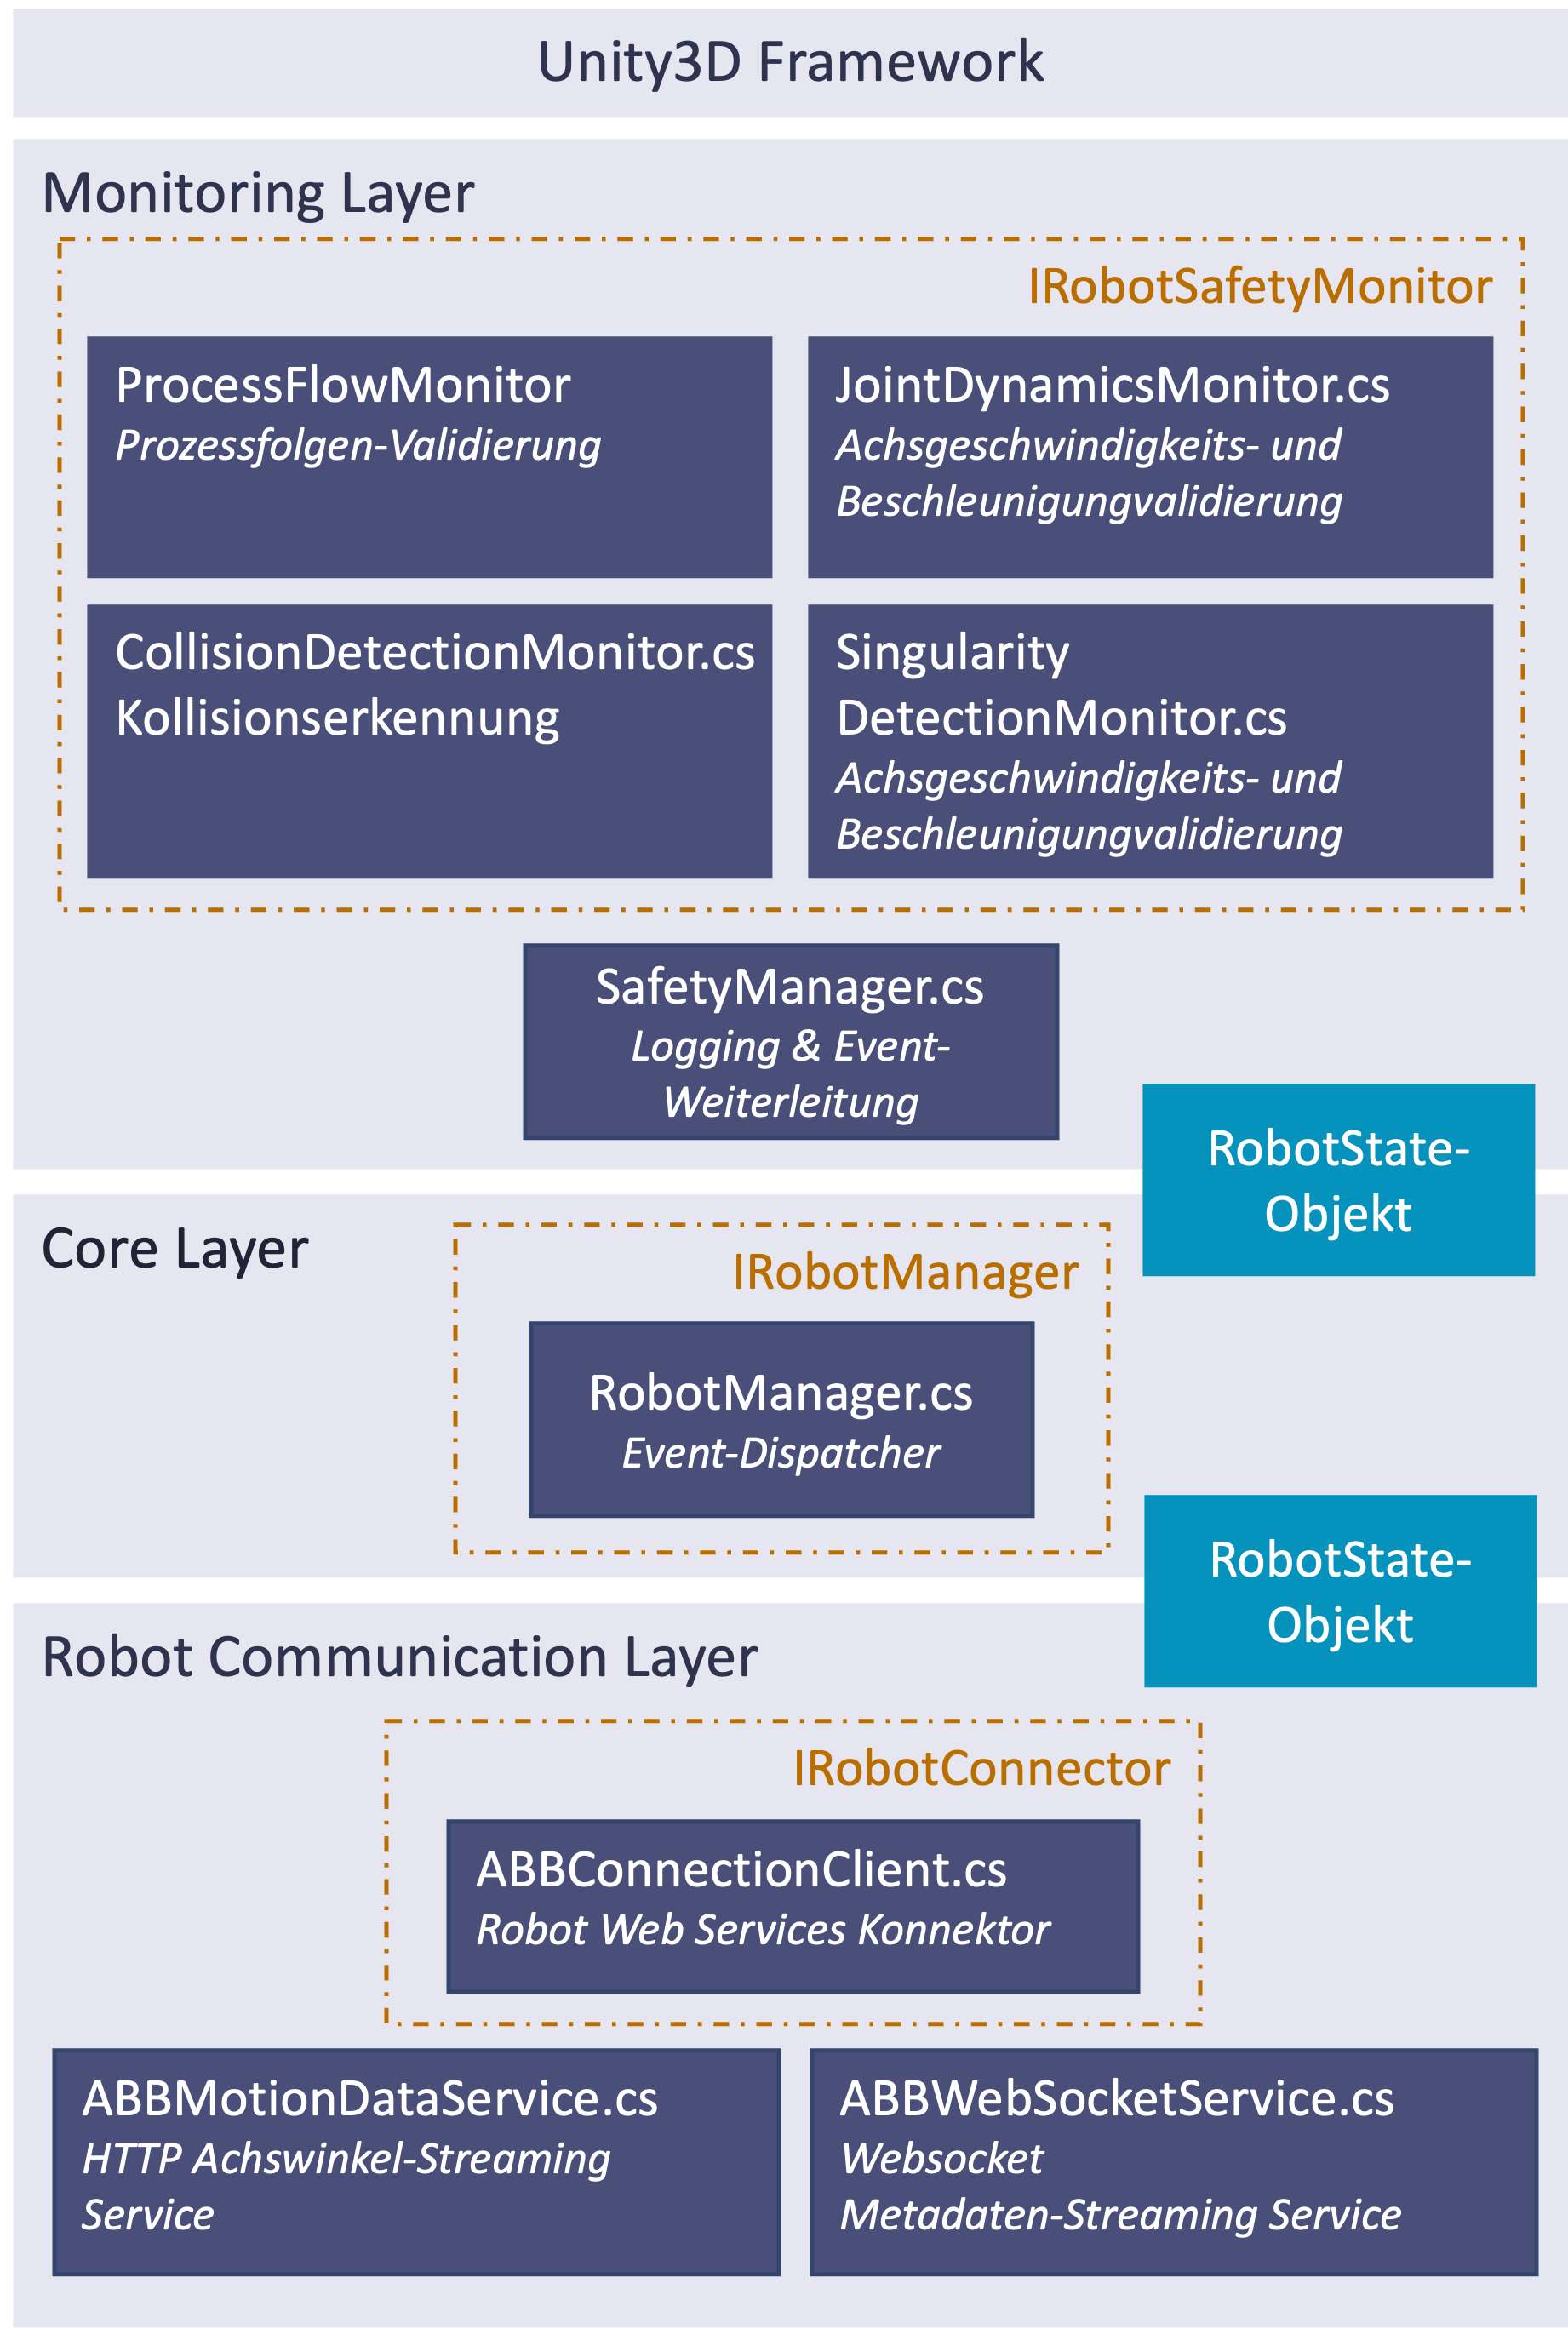
\includegraphics[width=10cm]{figures/LayerArchitekturFramework.png}
	\caption{Schichtenarchitektur des Frameworks. Orange umrandete Module implementieren formalisierte Interfaces (\texttt{IRobotSafetyMonitor}, \texttt{IRobotConnector}). Das \texttt{RobotState}-Objekt dient als gemeinsame Datenstruktur zwischen den Schichten.}
	\label{fig:layer_architecture}
\end{figure}

Die Architektur gliedert sich in vier logisch getrennte Schichten:

\begin{enumerate}
	\item \textbf{Unity3D Framework}: Bereitstellung der Simulationsumgebung und Physics-Engine
	\item \textbf{Monitoring Layer}: Implementierung der Sicherheitsmonitore
	\item \textbf{Core Layer}: Zentrales State-Management und Event-Koordination
	\item \textbf{Robot Communication Layer}: Adapter für herstellerspezifische Robotersteuerungen
\end{enumerate}


\subsection{Unity3D Framework (Simulationsschicht)}
Diese Schicht stellt ausschließlich die Simulationslaufzeit bereit (Szene, Physik, Rendering) und ist in der Anwendungslogik gekapselt. Architekturprinzip: \emph{Framework außen, Domäne innen}; der Zugriff erfolgt ausschließlich über wohldefinierte Adapter und Abstraktionen, nicht durch direkte Engine-Aufrufe in den Monitoren (\vglcite[293\psq]{gamma1994}, \vglcite{martin2003}).

\textbf{Verantwortlichkeiten:}
(i) Bereitstellung des Taktgebers für Zustandsupdates,
(ii) Ausführung asynchroner Tasks (Update-Loop),
(iii) Host für Adapter (z.\,B. \texttt{IRobotConnector}).

\subsection{Monitoring Layer}
Die Monitore kapseln die Erkennung jeweils eines Fehlertyps als \emph{Policy} über dem Roboterzustand. Jeder Monitor implementiert \texttt{IRobotSafetyMonitor} und ist damit austauschbar erweiterbar (\vglcite{martin2003}). Ereignisse werden ausschließlich \emph{event-getrieben} erzeugt und nach unten an den Core weitergereicht (\vglcite[97\psqq]{Hohpe2003}).

\textbf{Verantwortlichkeiten:}
(i) domänenspezifische Prüfregeln (Kollision, Singularität, Prozessfolge, Dynamik),
(ii) Erzeugung normalisierter \texttt{SafetyEvent}s,
(iii) keine Engine- oder IO-Abhängigkeiten.

\textbf{Wesentliche Typen:}
\texttt{IRobotSafetyMonitor}, \texttt{SafetyEvent}, \texttt{SafetySeverity}.

% Mini-Listing: reine Signatur, kurz halten
\begin{figure}[H]
	\inputminted[fontsize=\footnotesize,breaklines]{csharp}{code-snippets/IRobotSafetyMonitor.cs}
	\caption{Kerninterface des Monitoring Layers (\texttt{IRobotSafetyMonitor})}
\end{figure}

Der \texttt{RobotManager} im Core Layer fungiert als zentraler Event-Dispatcher,
der Zustandsänderungen an alle registrierten Monitoring-Komponenten propagiert.
Diese Implementierung des Observer Patterns \vglcite[293-303]{Gamma1994}
ermöglicht eine lose Kopplung zwischen den Komponenten: Die Sicherheitsmonitore
müssen lediglich das \texttt{IRobotSafetyMonitor}-Interface implementieren und
können zur Laufzeit dynamisch registriert oder entfernt werden, ohne andere
Systemteile zu beeinflussen.

Die in Abbildung \ref{fig:layer_architecture} orange markierten Module
definieren standardisierte Interfaces, die als Verträge zwischen den Schichten
dienen. Diese Interface-basierte Abstraktion realisiert das Open-Closed
Principle \vglcite{Martin2003}: Neue Robotertypen können durch Implementierung
des \texttt{IRobotConnector}-Interfaces integriert werden, ohne den Core Layer
zu modifizieren. Analog können zusätzliche Sicherheitsmonitore über das
\texttt{IRobotSafetyMonitor}-Interface hinzugefügt werden. Diese
Architekturentscheidung gewährleistet, dass das System für Erweiterungen offen
bleibt, während die Kernfunktionalität unverändert bleibt.

Die Kommunikation zwischen den Schichten erfolgt ereignisgesteuert über das
\texttt{RobotState}-Objekt als gemeinsame Datenstruktur. Die Communication Layer
aktualisiert kontinuierlich den Roboterzustand durch WebSocket-Events für
Metadaten und HTTP-Polling für Bewegungsdaten. Der \texttt{RobotManager}
verteilt diese Zustandsänderungen asynchron an alle registrierten Observer.
Diese Event-Driven Architecture \vglcite[97\psqq]{Hohpe2003} adressiert die
Echtzeitanforderungen industrieller Robotersysteme: Kritische
Sicherheitsereignisse wie Kollisionen werden mit minimaler Latenz erkannt und
priorisiert verarbeitet, während weniger kritische Ereignisse gepuffert werden
können.

Der \texttt{SafetyManager} aggregiert die von den Monitoren generierten
Sicherheitsereignisse und implementiert eine kontextabhängige Logging-Strategie.
Bei laufendem Roboterprogramm werden detaillierte JSON-Logs für spätere Analyse
erstellt, während im Idle-Zustand nur kritische Ereignisse in die Konsole
geloggt werden. Diese Differenzierung optimiert sowohl die Performance als auch
die Nachvollziehbarkeit von Sicherheitsvorfällen.

Die gewählte Schichtenarchitektur ermöglicht die unabhängige Entwicklung und
Testung einzelner Komponenten. Horizontale Erweiterungen (neue Monitore) und
vertikale Erweiterungen (neue Robotertypen) können ohne Seiteneffekte auf
bestehende Komponenten implementiert werden.

\subsection{Robot Communcation Layer}
Die Robot Communication Layer organisiert die Kommunkation mit der zugrundeliegenden Robotersteuerung und
implentiert eine Interface des Typs IRobotConnector. Als Verbindungsclient
zwischen Unity und externer Schnittstelle des Robotersystems implementiert
dieser eine IRobotConnector Interface, welche als Vorlage für eine Anbindung an
eine Robotersteuerung jedes Typs fungiert und standartisierte Methoden
implementiert:

\begin{figure}[H]
	\inputminted[fontsize=\footnotesize]{csharp}{code-snippets/IRobotConnector.cs}
	\caption{Implementierung der IRobotConnector-Interface als Verbidung zwischen
		RobotState und Roboter-Controller}
\end{figure}
\noindent
Eine Interface lässt sich anhand dieses Beispiels in \textbf{3
	Funktionsbereiche} aufteilen: Events, Attribute und Methoden.\\

\noindent
Die Interface definiert \textbf{Events (Aktionen)} die bei definierten Zustandsänderungen
in der Laufzeit ausgeführt werden. Andere Bestandteile des Framework sind in der
Lage, ein Event zu abonnieren und eine Methode registieren, welche ausgeführt
werden soll, wenn dieses Event auftritt. Ist dies der Fall, wird das
entsprechende Modul über die Änderung benachrichtigt und bekommt gegebenfalls
neue Daten zur Verfügung gestellt. Diese event-getriebene Kommunikation sorgt
dafür, dass einerseits alle Komponenten proaktiv auf den neusten Stand der Daten gebracht
und gehalten werden, andererseits aber keine ressourcenblockierenden Prozesse
ausgeführt werden müssen, um gegebenfalls Statusänderungen abzufragen.\\

\noindent
Weiterführend definiert die Interface IRobotConnector \textbf{Attribute}, welche den
aktuellen Verbindungsstatus (verbunden = \texttt{true}, getrennt = \texttt{false}) speichern sowie das
State-Objekt des Roboters. Definiert durch die schreibgeschützten, automatisch
implementierte Eigenschaft mit einem Getter \textit{\{ get; \}} können Attribute
auch von ausserhalb des RobotConnectors abgefragt werden, jedoch nicht
überschrieben.\\

\noindent
Zuletzt gibt die Interface die Methoden \textit{\textbf{Connect}} und \textit{\textbf{Disconnect}}
vor, welche hier die wichtigsten Methoden zum Verbinden und
Trennen von der jeweiligen Robotersteuerung darstellen.

Als initiale Komponente wird eine Verbindung zum
Controller eines Roboters benötigt, um den Roboter in Unity emulieren zu können
und Daten zu verarbeiten. Dazu wird hier mittels eines HTTP-Clients zur
Schnittstelle des RobotStudioSDKs über die API RobotWebServices (RWS) eine
Verbindung aufgebaut. Die Verbindung zu RobotWebServices ensteht durch einen
HTTP-Client und der Authentifizierung mit in RobotStudio festgelegten
Zugangsdaten. Anschliessend kann über einen erhaltenen Cookie die Verbindung
aufrecherhalten werden und aktuelle Daten über den Roboter sowohl abgefragt,
also auch der Roboter selbst gesteuert werden.\vglcite{robotwebservices2025}

Die RWS-Schnittstelle bietet einerseits die Möglichkeiten,
aktuellen Achswinkel und TCP-Werte (Tool Center Point) abzurufen, als auch
weitere Metadaten, wie das aktuell laufende Programm, den aktuellen Motorstatus
oder auch die Codezeile, welche aktuell vom Programmzeiger ausgeführt wird.
Weiterführend bietet RWS die Möglichkeit, die aktuelle digitale und analoge
Signale abzurufen, was nötig ist, um den Greifer steuern zu können.

Bei den oben genannten Daten mit Ausnahme der Achswinkel handelt es sich um
Paramenter, welche sich im Laufe eines Programmablaufs vergleichsweise selten
verändern. Daher wird hier auf den Websockets-Endpunkt von RWS zugegriffen, um
innerhalb einer Duplex-Kommunikation sich verändernende Signale oder auch
Programmstati zu empfangen. Dazu wird mithilfe des HTTP-Clients eine Anfrage zur
Subscription auf verschiedene Parameter (bspw. den ProgrammPointer) gestellt,
und anschliessend eine Websockets-Session aufgebaut. Die Achswinkel werden
zeitgleich über eine asynchron endlosen Task in einer in Unity definierbaren
Frequenz abgefragt.

Der Client implementiert dabei die Interface IRobotConnector und gibt ein
RobotState-Objekt mit den empfangenen Daten an den RobotManager weiter, welcher hier
als zentraler Koordinator des aktuellen RobotState fungiert.

\noindent
\paragraph{Event-Driven Architecture}
as System nutzt ein durchgängiges Event-System für lose Kopplung:
\begin{itemize}
	\item \texttt{OnRobotStateUpdated}: Zustandsänderungen
	\item \texttt{OnConnectionStateChanged}: Verbindungsstatus
	\item \texttt{OnSafetyEventDetected}: Sicherheitsereignisse
	\item \texttt{OnMotorStateChanged}: Motorstatusänderungen
\end{itemize}

\paragraph{SafetyEvent und RobotStateSnapshot}
Als für die Auswertung der Simulationsergebnisse relevantes Teil des Frameworks
wird eine SaftetyEvent-Objekt implementiert. Jedes Mal, wenn ein Ereignis,
welches mit der tatsächlichen Simluation eines Roboterpgrogramms zusammenhängt,
auftritt, wird ein SafetyEvent instanziert. Dieses wird initial von der
jeweiligen überwachenden Komponente (einem SafetyMonitor) instanziert und mit
dem aktuellsten RobotState als unveränderliches Objekt (RobotStateSnapshot) befüllt.
Weiterführend erhält es vom jeweiligen SafetyMonitor variierende
Kontextinformationen, die später für die Auswertung des Ereignisses verwendet
werden. Zusammenfassend bestehn ein SafetyEvent aus folgenden Komponenten:
\begin{itemize}
	\item \textbf{SafetyEvent}: Unveränderliches Value Object für Sicherheitsereignisse
	\item \textbf{RobotStateSnapshot}: Immutable Zustandserfassung zum Ereigniszeitpunkt
	\item \textbf{Ereignistypen}: Info, Warning, Critical mit konfigurierbaren Schwellwerten
	\item \textbf{Kontextdaten}: Vollständige Roboterzustandserfassung für Forensik
\end{itemize}
\noindent


\section{Implementierung der Monitore zur Fehlererkennung}
\label{sec:implementierungMonitore}

Zur Orientierung sind die im Framework implementierten Monitore in
Tabelle~\ref{tab:monitor_overview_arch} zusammengefasst. Die Tabelle zeigt Ziel,
Eingabedaten und Art der generierten Events.

\begin{table}[H]
  \centering
  \small
  \begin{tabularx}{\textwidth}{lXX}
    \toprule
    \textbf{Monitor}        & \textbf{Ziel}
    & \textbf{Eingabedaten / Events} \\
    \midrule
    Prozessfolgen           & Einhaltung der definierten Abfolge von
    Arbeitsschritten               &
    Aktuelle Sequenz, Soll-Sequenz / Event bei Abweichung
    \\
    \addlinespace
    Kollisionen             & Erkennung von Zusammenstößen zwischen
    Roboter und Umgebung            &
    Geometrieinformationen / Event mit Schweregrad und beteiligten
    Objekten                                                          \\
    \addlinespace
    Singularitäten          & Detektion von \mbox{Handgelenks-,} Ellbogen- und
    Schulter-Singularitäten              &
    Gelenkwinkel, Jacobi-Matrix / Entering- und Exiting-Events mit
    Manipulierbarkeit                                                      \\
    \addlinespace
    Gelenkgeschwindigkeiten & Überwachung von Winkel-,
    Geschwindigkeits- und Beschleunigungsgrenzen &
    Gelenkwinkel / exceeded- und resolved-Events bei
    Grenzwertverletzung
    \\
    \bottomrule
  \end{tabularx}
  \caption{Überblick über die implementierten Monitore im Framework}
  \label{tab:monitor_overview_arch}
\end{table}

\subsection{Prozessfolgen}
\label{ssec:Prozessfolgen}
% Überprüfung der korrekten Abfolge von Aktionen...
User Input: Simulationsumgebung und Verbindung zu Robot Studio

Wie kann ich Prozessfolgen überprüfen? Prozessfolge: Folge and Arbeitsschritten
eines Arbeitsprozesses, hier Roboter -> Was wird in welcher Reihenfolge wohin
bewegt? Wie kann ich das Messen? - Bewegt sich das Werkstück von Position Start
zu Position Ziel? - Bewegen sich die Werkstücke in der richtigen Reihenfolge
von Start zu Ziel? Benötigt: Definition von Start \& Zielpositionen einzelner
Werkstücke

\subsection{Kollisionen}
\subsubsection{Theoretische Grundlagen}

Kollisionen eines Roboters mit Objekten im Arbeitsraum stellen eine zentrales
Problem beim Neuentwurf und der Testung neu entwickelten Codes dar. Kollidiert
ein industrieller Roboter unvorhergesehen mit seinem Arbeitsraum, kann dies im
schlimmsten Fall zu einem Ausfall des am Produktionsschrit beteiligen Roboters
\subsubsection{Implementierung}



\subsection{Singularity Detection Monitor} \label{ssec:Singularitaeten}
Im Folgenden wird der Singularity Detection Monitor zur Erkennung von
singulären Gelenkpositionen des Roboters näher erläutert. Ziel ist es,
Handgelenks-, Ellbogen- und Schulter-Singularitäten festzustellen und beim
Auftreten Events mit relevanten Informationen wie Achswinkeln, Nähe zur
Singularität sowie verbleibende Manipulierbarkeit des Roboters auszugeben.

\subsubsection{Theoretische Grundlagen der Singularitätsdetektion}
\label{sssec:Theorie_Singularitaeten}
Kinematische Singularitäten stellen ein fundamentales Problem in der
Robotersteuerung dar und treten auf, wenn die Jacobi-Matrix des Roboters ihren
vollen Rang verliert. In diesen Konfigurationen verliert der Roboter die
Fähigkeit, sich in bestimmte Richtungen im kartesischen Raum zu bewegen, was zu
Kontrollverlust und potentiell gefährlichen Situationen führen
kann.\vglcite{siciliano2016robotics}

Eine kinematische Singularität tritt auf,
wenn die Jacobi-Matrix $\mathbf{J}(\boldsymbol{\theta})$, welche des Roboters
ihren vollen Rang verliert:
\begin{equation}
  \text{rank}(\mathbf{J}(\boldsymbol{\theta})) < \min(m, n)
  \label{eq:singularity_condition}
\end{equation} wobei
$\mathbf{J}(\boldsymbol{\theta}) \in \mathbb{R}^{m \times n}$ die Jacobi-Matrix,
$\boldsymbol{\theta}$ der Gelenkwinkelvektor, $m$ die Anzahl der Freiheitsgrade
im kartesischen Raum und $n$ die Anzahl der Robotergelenke darstellt.

Die Jacobi-Matrix beschreibt die Beziehung zwischen Gelenkgeschwindigkeiten
$\dot{\boldsymbol{\theta}}$ und kartesischen Geschwindigkeiten des TCP
$\mathbf{v}$:
\begin{equation} \mathbf{v} = \mathbf{J}(\boldsymbol{\theta})
  \dot{\boldsymbol{\theta}} \label{eq:jacobian_velocity}
\end{equation}

Tritt eine Singularität auf, so wird die Jacobi-Matrix singulär:
\begin{equation} \det(\mathbf{J}) = 0 \label{eq:jacobian_singularity}
\end{equation} Dadurch wird die inverse Kinematik nicht
eindeutig lösbar ist und es können theoretisch unendliche
Gelenkgeschwindigkeiten auftreten.\vglcite{nakamura1991advanced}

\subsubsection{Frameworkspezifisches Vorgehen}
Im Rahmen der praktischen Implementierung wird hier ein auf Schwellwerten und
absoluten sowie winkelbasierten Entfernungen zur Singularität angewendet. Durch
die Anwendung der rein mathematischen Definition ließe sich zwar jede beliebige
Singularität in einer seriellen Kinematik erkennen, jedoch bleiben die
betroffenen Gelenke und Art der Singularität ungewiss und müssten iterativ
bestimmt werden. Daher wird hier eine pragmatische Berechnungsmethodik
verwendet.

Für serielle Robotermanipulatoren mit sechs Freiheitsgraden, wie den hier
verwendeten ABB IRB 6700, können drei primäre Singularitätstypen unterschieden
werden: Schultersingularitäten, Ellbogensingularitäten und
Handgelenksingularitäten.\vglcite{spong2006robot}

\paragraph{Schultersingularitäten} treten auf, wenn sich das
Handgelenkszentrum (Schnittpunkt der Achsen 4, 5, 6) direkt über oder nahe der
Rotationsachse des ersten Gelenks befindet:

\begin{equation}
  \sqrt{x_{wc}^2 + y_{wc}^2} < \epsilon
  \label{eq:shoulder_singularity}
\end{equation}

wobei $(x_{wc}, y_{wc})$ die Position des Handgelenkszentrums in der XY-Ebene
und $\epsilon$ der Singularitätsschwellenwert ist.

\paragraph{Ellbogensingularitäten} treten auf, wenn der Roboter die
Grenzen seines
Arbeitsraums erreicht. Dies geschieht typischerweise bei vollständig
ausgestreckter oder eingeklappter Konfiguration. Beim
Knickarmrobotern wie dem IRB 6700
verläuft die Rotationsachse des vierten Gelenks nicht direkt durch
den Ursprung vom
dritten Gelenk, sondern ist durch eine Translation verschoben. Das impliziert,
dass die vollständige Streckung des Armes nicht durch einen Winkel
von $0^\circ$ bzw.
$180^\circ$ auftritt. Hier lässt sich allgemeiner der Zusammenhang der Vektoren
zwischen Gelenk 2 und 3 sowie 2 und 5 anwenden:

\begin{equation}
  \theta = \angle(\vec{v}_{23}, \vec{v}_{25}) \approx 0^\circ \text{
  oder } \theta \approx 180^\circ
  \label{eq:elbow_singularity}
\end{equation}

wobei:
\begin{align}
  \vec{v}_{23} & = \vec{p}_3 - \vec{p}_2 \\
  \vec{v}_{25} & = \vec{p}_5 - \vec{p}_2
\end{align}

mit $\vec{p}_i$ als Position des Gelenks $i$. Die Singularitätsbedingung lautet:
\begin{equation}
  \theta < \epsilon \quad \text{oder} \quad \theta > 180^\circ - \epsilon
\end{equation}

\paragraph{Handgelenksingularitäten} treten auf, wenn die Rotationsachsen der
letzten drei Gelenke (Gelenke 4, 5, 6) kollinear werden. Dies tritt
typischerweise auf, wenn $\theta_5 = 0^\circ$ oder $\theta_5 =
180^\circ$. Mathematisch
beschrieben durch:

\begin{equation}
  \mathbf{z}_4 \parallel \mathbf{z}_6 \text{ oder } |\mathbf{z}_4
  \cdot \mathbf{z}_6| \approx 1
  \label{eq:wrist_singularity}
\end{equation}

wobei $\mathbf{z}_i$ die Rotationsachse (Z-Achse) des $i$-ten Gelenks im
Weltkoordinatensystem darstellt. Beispielhaft ist das Auftreten einer
Handgelenkssingularität in Abbildung~\ref{figure:wristSingularity}
in Unity3D.

\subsubsection{Manipulierbarkeitsindex (Yoshikawa-Maß)} Der von Yoshikawa
\cite{yoshikawa1985manipulability} eingeführte Manipulierbarkeitsindex ist eine
der am häufigsten verwendeten Metriken:
\begin{equation}
  \mu(\boldsymbol{\theta}) =
  \sqrt{\det(\mathbf{J}(\boldsymbol{\theta})\mathbf{J}^T(\boldsymbol{\theta}))}
  \label{eq:yoshikawa_measure}
\end{equation}

Für quadratische Jacobi-Matrizen vereinfacht sich dies zu:
\begin{equation}
  \mu(\boldsymbol{\theta}) = |\det(\mathbf{J}(\boldsymbol{\theta}))|
  \label{eq:yoshikawa_simplified}
\end{equation}

Der Index nimmt Werte zwischen 0 (Singularität) und einem maximalen Wert an,
wobei höhere Werte bessere Manipulierbarkeit indizieren. Die Robotik-Literatur
bietet verschiedene Ansätze zur Behandlung von Singularitäten, die sich in
präventive und reaktive Strategien unterteilen lassen. Um diese in der Praxis
anzuwenden, müssen jedoch teilweise numerische Auswertungen durchgeführt werden,
um Schwellwerte zu erfassen. Daher kommen diese hier nicht zum Einsatz.

Zur zusätzlichen Charakterisierung wird jedoch die Yoshikawa-Manipulierbarkeit
berechnet, da der Wert als Kennzahl für die Nähe zu einer Singularität verwendet
werden kann. Er wird in den Ergebnissen in Kapitel
\ref{sec:singularityauswertung} aufgeführt.

\begin{figure}[H]
  \centering
  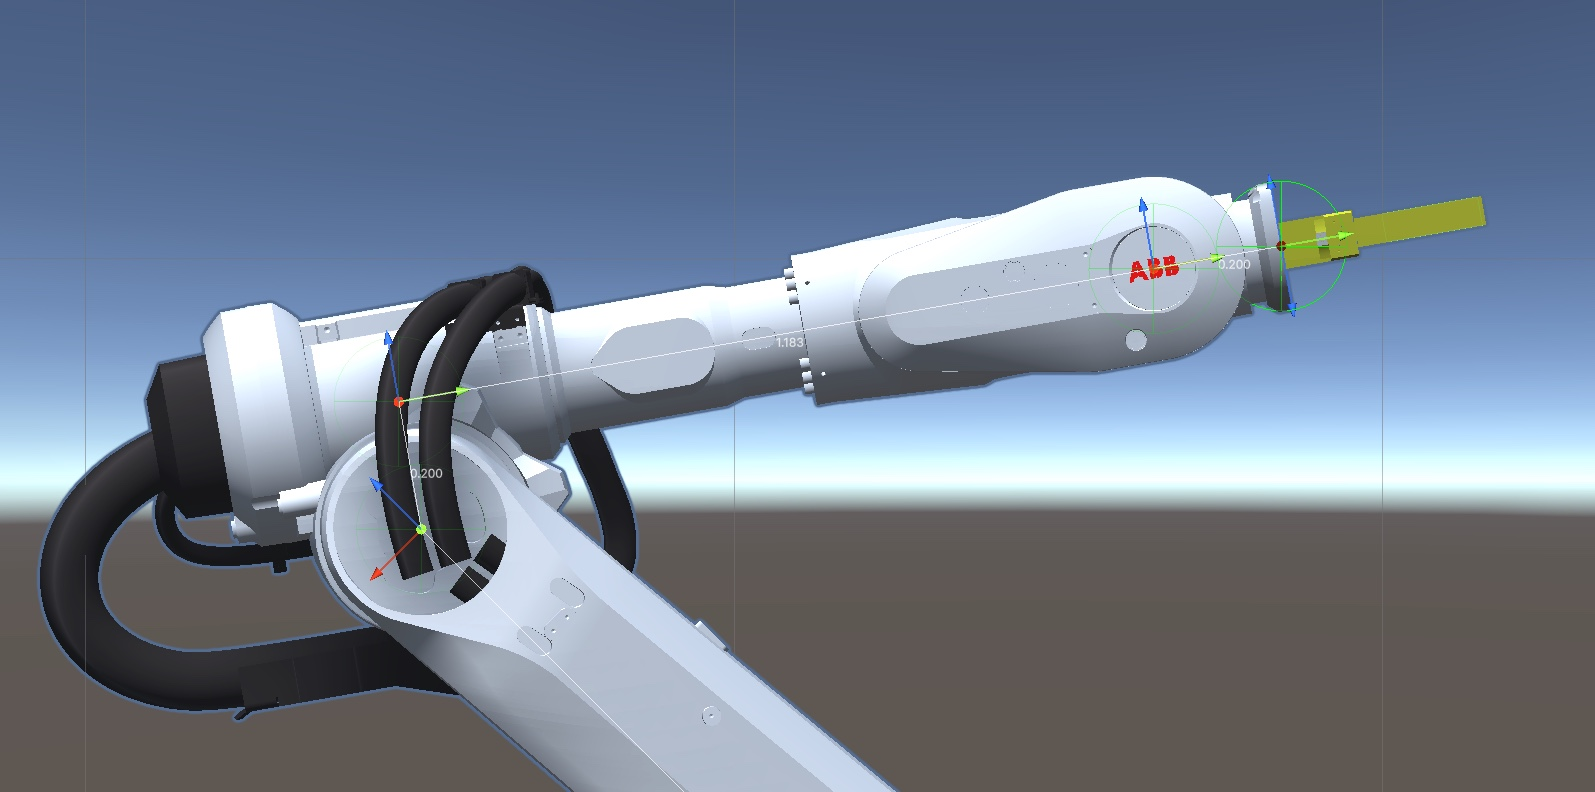
\includegraphics[width=\linewidth]{Figures/wristSingularityScreenshot.jpg}
  \caption{Screenshot einer Handgelenksingularität in Unity mit farbig
  dargestellten Koordinatensystemen der Denavit-Hartenberg-Transformationen }
  \label{figure:wristSingularity}
\end{figure}

\subsubsection{Praktisches Vorgehen}
Nachfolgend werden die Schritte 1 bis 4 zur Prüfung des Vorliegens
einer Singularität dargestellt.

\paragraph{Schritt 1: Positionsberechnung und Achsentransformation}~\\
Die Positionen der relevanten Gelenke werden durch die Anwendung der
Vorwärtstransformation nach Denavit-Hartenberg (DH)
berechnet\vglcite{denavit1955}:
\begin{equation}
  \vec{p}_i = \text{DH}(\theta_1, \ldots, \theta_i) \quad \text{für }
  i = 2, 3, 5
  \label{eq:position_calculation}
\end{equation}

Die Rotationsachsen werden aus den Transformationsmatrizen extrahiert:
\begin{equation}
  \mathbf{z}_i = \mathbf{T}_i[:3, 2] \quad \text{für } i = 1, 4, 6
  \label{eq:axis_extraction}
\end{equation}

\paragraph{Schritt 2: Singularitätsanalyse}~\\
Für jeden Singularitätstyp wird die entsprechende Bedingung überprüft:
\begin{itemize}
  \item \textbf{Schultersingularität:}
    \begin{equation}
      d_{wc} = \sqrt{x_{wc}^2 + y_{wc}^2}
    \end{equation}
    wobei $(x_{wc}, y_{wc})$ die Position des Handgelenkszentrums in
    der XY-Ebene ist.

  \item \textbf{Ellbogensingularität:}
    \begin{equation}
      \theta_{elbow} = \angle(\vec{p}_3 - \vec{p}_2, \vec{p}_5 - \vec{p}_2)
    \end{equation}

  \item \textbf{Handgelenksingularität:}
    \begin{equation}
      c_{46} = |\mathbf{z}_4 \cdot \mathbf{z}_6|
    \end{equation}
\end{itemize}

\paragraph{Schritt 3: Schwellwertvergleich}~\\
\begin{table}[H]
  \centering
  \begin{tabular}{l l l}
    \hline
    \textbf{Singularitätstyp} & \textbf{Beispiel-Schwellwert}      &
    \textbf{Bedingung}                            \\
    \hline
    Schulter                  & $\tau_{\text{shoulder}} = 100$ mm  &
    $d_{wc} < \tau_{\text{shoulder}}$             \\
    Ellbogen                  & $\tau_{\text{elbow}} = 5^{^\circ}$ &
    $\theta_{elbow} < \tau_{\text{elbow}}$ oder   \\
    &                                    & $\theta_{elbow} >
    180^\circ - \tau_{\text{elbow}}$ \\
    Handgelenk                & $\tau_{\text{wrist}} = 5^{^\circ}$ &
    $c_{46} > \tau_{\text{wrist}}$                \\
    \hline
  \end{tabular}
  \caption{Singularitätsschwellwerte und Detektionsbedingungen}
  \label{tab:singularity_thresholds}
\end{table}

\paragraph{Schritt 4: Manipulierbarkeitsberechnung}~\\
Für detektierte Singularitäten wird ein approximierter Manipulierbarkeitsindex
nach Yoshikawa berechnet:

\begin{equation}
  w = \sqrt{\det(\mathbf{J}(\theta)\mathbf{J}^T(\theta))}
  \label{eq:manipulability}
\end{equation}

Ein kleiner Wert von $w$ indiziert die Nähe zu einer singulären Konfiguration.
Das entwickelte Framework implementiert eine winkelbasierte
Singularitätsdetektion, die geometrische Eigenschaften der Roboterkinematik
direkt nutzt, anstatt auf rechenintensive Jacobi-Matrix-Berechnungen angewiesen
zu sein. Die achsenbasierte Methode basiert auf der Erkenntnis, dass
Handgelenks- und Ellbogensingularitäten geometrisch durch die
Kollinearität von Rotationsachsen
charakterisiert werden können. Schultersingularitäten werden analog durch die
Entfernung des ersten Gelenks zum Handgelenkzentrum in der XY-Ebene
festgestellt.

\subsubsection{Konkrete Implementierung der Detektionsmethoden}
\label{sssec:Implementierung_Detektionsmethoden}
Die Implementierung des \texttt{SingularityDetectionMonitor} nutzt die
Vorwärtskinematik des Preliy Flange Frameworks zur Berechnung der
Gelenkpositionen. Die zentrale Methode \texttt{ComputeJointPosition} berechnet
die kartesische Position eines beliebigen Gelenks durch sukzessive Anwendung
der Denavit-Hartenberg-Transformationsmatrizen (vgl.
Abbildung~\ref{listing:forwardKinematic}).

\begin{figure}[H]
  \inputminted[fontsize=\footnotesize]{csharp}{code-snippets/CalculateJointPos.cs}
  \caption{Vorwärtskinematik zur Positionsberechnung}
  \label{listing:forwardKinematic}
\end{figure}

Die Methode \texttt{ComputeJointPosition} in Abbildung
\ref{listing:forwardKinematic} implementiert die klassische
Vorwärtskinematik durch
Multiplikation homogener Transformationsmatrizen. Jede Matrix $\mathbf{T}_i$
wird aus den DH-Parametern $(\alpha_i, a_i, d_i, \theta_i)$ konstruiert, wobei
$\theta_i$ der aktuelle Gelenkwinkel plus einem konstanten Offset ist. Die
resultierende Transformationsmatrix beschreibt die Position und Orientierung des
Gelenks im Basiskoordinatensystem.\\

Das Framework nutzt Unitys \texttt{Matrix4x4}-Klasse für die
Transformationsberechnungen und die \texttt{GetPosition()}-Methode zur
Extraktion der Translationskomponente. Die Koordinatentransformation zwischen
dem DH-Parametersystem und Unitys linkshändigem Y-up Koordinatensystem wird
dabei durch die Methode \texttt{HomogeneousMatrix.CreateRaw()} des
Flange-Frameworks transparent gehandhabt. Das ermöglicht eine nahtlose
Integration der mathematischen Robotik-Konzepte in die Unity-Umgebung, während
die Echtzeitfähigkeit durch eventgetriebene Berechnung gewährleistet ist.
Bei der Detektion einer Singularität bzw. dem Unterschreiten des im Unity-Editor
definierten Grenzwertes wird ein \texttt{SafetyEvent}-Objekt
instanziert und an die
\texttt{SafetyMonitor} Klasse weitergegeben. Darin werden zusätzlich
Event-Metadaten zu den
Daten der Gelenkwinkelabstände ausgegeben. Sobald der
kritische Bereich verlassen wurde, wird ein weiteres
\texttt{SafetyEvent} ausgegeben, um
den Bereich, in welcher die Singularität auftritt, abstecken zu können.


\subsection{Joint Dynamics Monitor}
\label{sssec:joint_dynamics_monitor}

\paragraph{Theoretische Grundlagen} Die Überwachung kinematischer Grenzwerte
während der Werkstückhandhabung stellt eines der zentralen Ziele des Frameworks dar. Die besondere Herausforderung in HTTP-basierten Systemen
liegt in der diskreten Datenakquisition mit Polling-Intervallen von 50-1000ms,
wodurch die numerische Differentiation zu erheblichen Instabilitäten
führt.

Geschwindigkeit $\dot{\theta}_i$ und Beschleunigung $\ddot{\theta}_i$ können folgendermassen aus der diskreten Zeitreihe approximiert werden:
\begin{equation}
	\dot{\theta}_i[k] = \frac{\theta_i[k] - \theta_i[k-1]}{\Delta t_k}, \quad
	\ddot{\theta}_i[k] = \frac{\dot{\theta}_i[k] - \dot{\theta}_i[k-1]}{\Delta t_k}
	\label{eq:discrete_derivatives}
\end{equation}

In der Praxis und nach initalem Testen hat sich herausgestellt, dass die
Berechnung dessen durch die untstetige Bewegung unrealistische Werte liefert.
Das hängt damit zusammen, dass der HTTP-Endpunkt des Robotercontrollers in
festgelegten Zeitabständen abgefragt wird und so die Gelenkpositionen des
Roboters erneuert werden. Bewegt sich der Roboter über eine bestimmte Strecke,
wird die von Unity lediglich als unstetige Bewegung mit theoretisch unendlich
grosser Geschwindigkeit wahrgenommen. Daher ist hier eine Glättung der Werte
nötig, um eine stetige Bewegung zu simulieren.

\paragraph{Mehrstufiger Filteransatz}
Zur Stabilisierung implementiert das Framework einen dreistufigen Filteransatz:

\begin{enumerate}
	\item \textbf{Exponential Moving Average (EMA):}
	      $\dot{\theta}_{i,\text{EMA}}[k] = \alpha \cdot \dot{\theta}_{i,\text{raw}}[k] + (1-\alpha) \cdot \dot{\theta}_{i,\text{EMA}}[k-1]$ mit $\alpha = 0.2$

	\item \textbf{Moving Window Average:}
	      $\dot{\theta}_{i,\text{MW}}[k] = \frac{1}{N} \sum_{j=0}^{N-1} \dot{\theta}_{i,\text{EMA}}[k-j]$ mit Fenstergröße $N = 8$

	\item \textbf{Outlier Rejection:}
	      $|\dot{\theta}_{i,\text{final}}[k] - \dot{\theta}_{i,\text{final}}[k-1]| \leq \tau_v \cdot \dot{\theta}_{i,\text{max}}$ mit $\tau_v = 0.2$
\end{enumerate}
\noindent
Durch die verwendete Glättung werden schnelle Änderungen in den Gelenkwerten
erst zeitverzögert sichtbar. Dies wirkt sich unmittelbar auf die Erkennung von
Geschwindigkeitsverletzungen aus, da der Monitor die Ereignisse nicht exakt im
Moment des Überschreitens ausgibt, sondern nach einigen Abtastungen.

\paragraph{Grenzwertdefinition} Die Grenzwerte werden aus den
Flange-Framework-Konfigurationen extrahiert oder manuell spezifiziert. Ein
Sicherheitsfaktor $\lambda = 0.8$ reduziert die nominellen Maximalwerte
präventiv. Für den ABB IRB 6700 ergeben sich beispielsweise
Geschwindigkeitsgrenzen von 88°/s für die Hauptachsen und bis zu 168°/s für das
Handgelenk.

\paragraph{Implementierung der Smoothing-Pipeline}
Die zentrale Smoothing-Methode kombiniert die Filteransätze:

\begin{figure}[H]
	\inputminted[fontsize=\footnotesize]{csharp}{code-snippets/SmoothVelocities.cs}
	\caption{Mehrstufige Smoothing-Pipeline zur Geschwindigkeitsberechnung}
	\label{listing:smoothing_pipeline}
\end{figure}

\noindent
Als weiteres Feature implementiert der Monitor eine Methode, welche sich an die
Update-Rate der State-Updates (also die Rate neuer Gelenkdaten) anpasst. So kann
garantiert werden, dass ein State nicht doppelt verarbeitet und so
beispielsweise die Geschwindigkeit falsch interpretiert wird, da es sich um den
immer gleichen State des Roboters handelt.\\

\noindent
Bei der Überschreitung der Schwellwerte wird der \texttt{SafetyMonitor}
mittels eines \texttt{SafetyEvents} benachrichtigt. Als zusätzliche Metadaten enthält
diese Meldung die Eventart (Geschwindigkeits oder
-Beschleunigungsüberschreitung) und die damit zusammenhängenden Schwellwerte und
aktuellen Werte. Da es in dem Rahmen vorkommen kann, dass hier die
Geschwindigkeit über einen längeren Zeitraum überschritten wird, gibt der
Monitor ebenfalls ein SafetyEvent aus, wenn die Geschwindigkeit unter den
gegebenen Schwelllwert sinkt.


\section{Testumgebung und -setup}
\label{sec:testumgebung}
Die Roboterzelle ist im Rahmen dieses Testszenarios als isolierter Arbeitsraum
mit mehreren Hindernissen, Begrenzungen und 3 semantischen Stationen aufgebaut.
Die vom Roboter zu bewältigenden Aufgaben beschränken sich dabei auf ein
Pick-and-Place-Szenario von Zylinderköpfen, dargestellt in
Abbildung~\ref{figure:arbeitsraum}.

\begin{figure}[H]
  \centering
  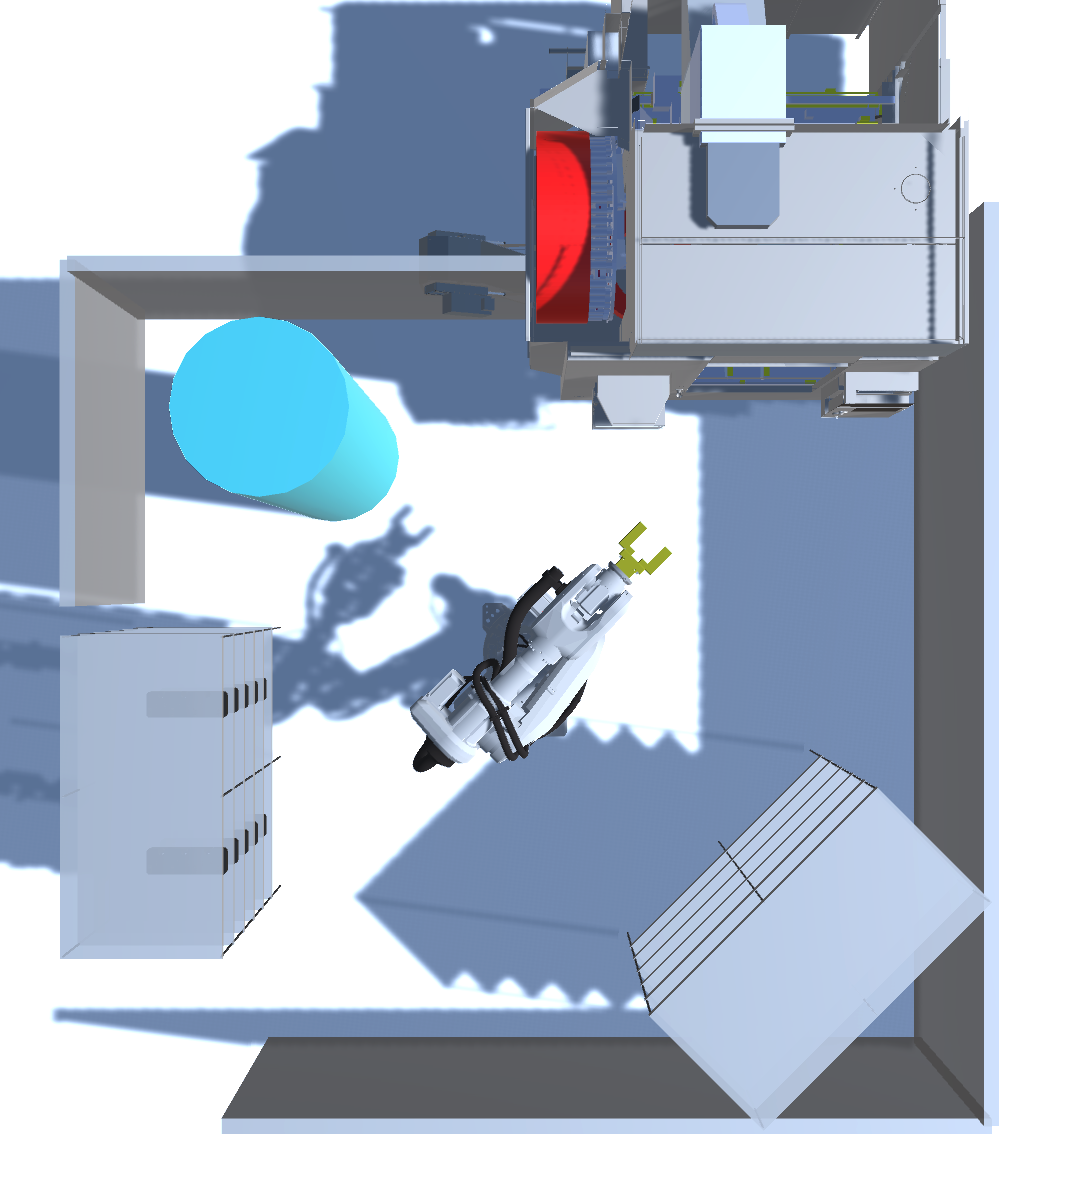
\includegraphics[width=10cm]{Figures/Roboterzelle.png}
  \caption{Arbeitsraum-Layout des Roboters in der Draufsicht mit Roboter in
  Home-Position}
  \label{figure:arbeitsraum}
\end{figure}

Das hierfür erstellte Layout sieht den Roboter in Zentrum des Arbeitsraumes auf
dem Boden stehend vor. Hindernisse, Begrenzungen und Stationen sind kreisförmig
um den Roboter angeordnet. In Abbildung
\ref{figure:arbeitsraum}
blau markiert, befindet sich eine Säule als künstliches Hindernis.
Links und rechts unten vom Mittelpunkt der Zelle aus befinden sich
zwei Regale als Teilelager. Oben befindet sich eine 5-Achs-Fräsmaschine mit
einer offenen Teileablage durch Entfernung der Schutztür zu
Vereinfachungszwecken dieses Szenarios. Der Arbeitsraum ist begrenzt durch
halbdurchsichtige Wände. Der Prozessablauf sieht vor, dass der Roboter
Zylinderköpfe aus dem linken Regal aufnimmt, diese in der Maschine ablegt, in
einer Warteposition auf die Beendigung der Bearbeitung wartet und anschliessend
das bearbeitete Teil aufnimmt, um es im rechten Regal abzulegen. Ein
beispielhafter Bearbeitungsprozess mit der 5-Achs-Fräsmaschine ist
hier das Bohren und Schneiden von Gewinden
in die Zylinderköpfe.

Der Aufbau und die Anordnung des Arbeitsraums ergibt sich aus den funktionalen
Anforderungen, die das Framework abdecken soll. Durch den relativ begrenzten
Raum müssen Bewegungspfade des Roboters an Hindernissen,
beispielsweise der Säule, vorbei
geplant werden und etwaige durch den Roboter gegriffene Werkstücke
mitberechnet werden. Weiterführend verringern die Regale den Bewegungsraum für
den Roboter zur Umorientierung vor sowie nach dem Aufnehmen und
Ablegen der Teile,
was zu einer erhöhten Wahrscheinlichkeit von Singularitäten führt. Die drei
semantischen Stationen sorgen dafür, dass sich hier Fehler im Prozessablauf
abbilden lassen. Die Achsgeschwindigkeiten lassen sich in diesem Szenario
ebenfalls beliebig variieren. Somit lassen sich alle funktionalen Anforderungen
des Frameworks innerhalb dieses vereinfachten Szenarios abbilden.

\subsubsection{Zylinderköpfe als Werkstücke}
Als Werkstücke werden hier Zylinderköpfe für V6-Motoren gewählt. Das Werkstück
bringt ein mit den Spezifikationen des ABB IRB 6700 übereinstimmendes Gewicht
mit und ist an den Seitenflächen durch einen Parallelgreifer gut greifbar. Die
Abmaße, des Zylinderkopfes sind Abbildung \ref{figure:cylinderhead}
zu entnehmen.

\begin{figure}[H]
  \centering
  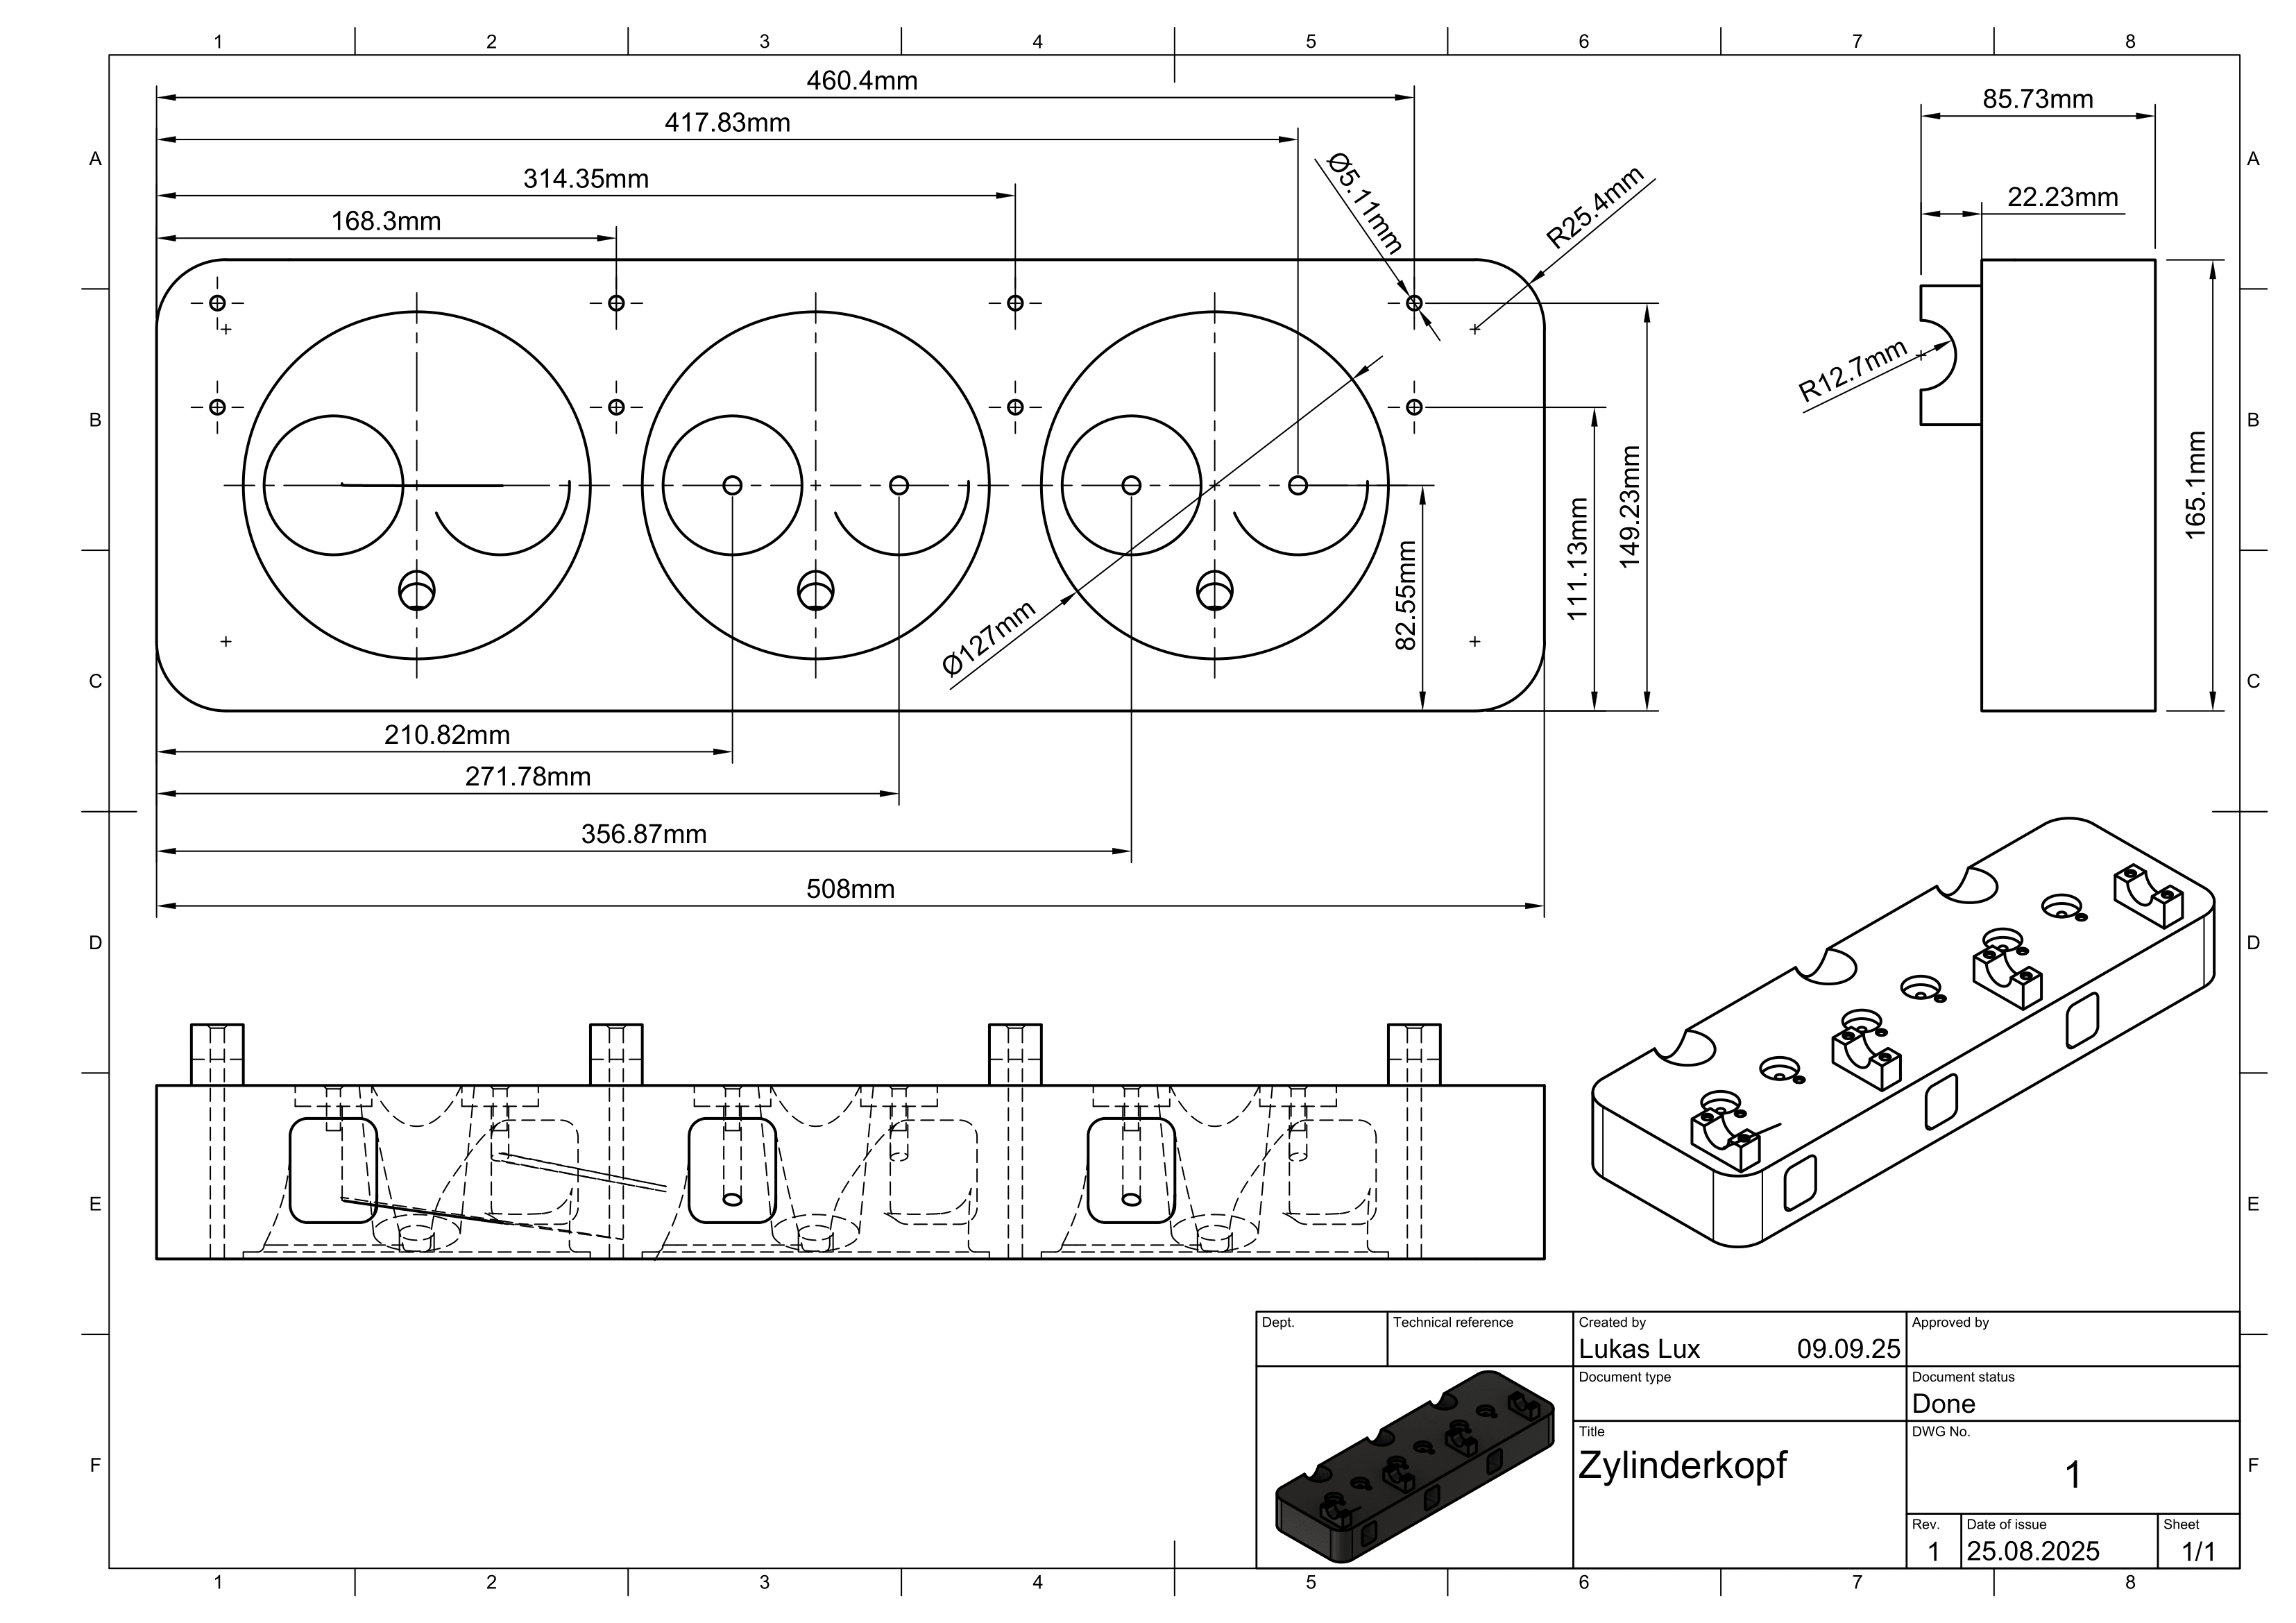
\includegraphics[width=\linewidth]{Figures/CyclinderHead-1.png}
  \caption{Technische Zeichung des verwendeten Zylinderkopfes, dargstellt
  mithilfe von Autodesk Fusion 360}
  \label{figure:cylinderhead}
\end{figure}

\subsubsection{Greiferauslegung}

Um das Werkstück sicher handhaben zu können, wird zusätzlich zum Roboter
ein End-Effektor benötigt, welcher das Werkstück sicher durch den Arbeitsraum
bewegen kann. Hierzu wird ein Parallelgreifer verwendet, welcher speziell zu
Handhabung des Zylinderkopfes ausgelegt wurde.
Da das Anforderungsprofil von End-Effektoren kaum normierbar und
werkstückabhängig ist, ist die Auslegung eines
spezifischen Greifers für die Handhabung individueller Werkstücke gängige
Praxis.\vglcite[91]{hesse2011}

Mithilfe eines Online-Konfigurationstools der Firma
SCHUNK\vglcite{schunk2025} ist es möglich, einen parametrisierten
Greifer auszulegen und als
3D-CAD-Modelle in verschiedenen Formaten herunterzuladen. Hier wurde
aufgrund der
Werkstückdimensionen ein Parallelgreifer der Baureihe PGN-Plus-P gewählt und die
Form der Greifbacken dem Werkstück entsprechend angepasst (siehe
Abbildung~\ref{figure:schunkGripper}).

\begin{figure}[H]
  \centering
  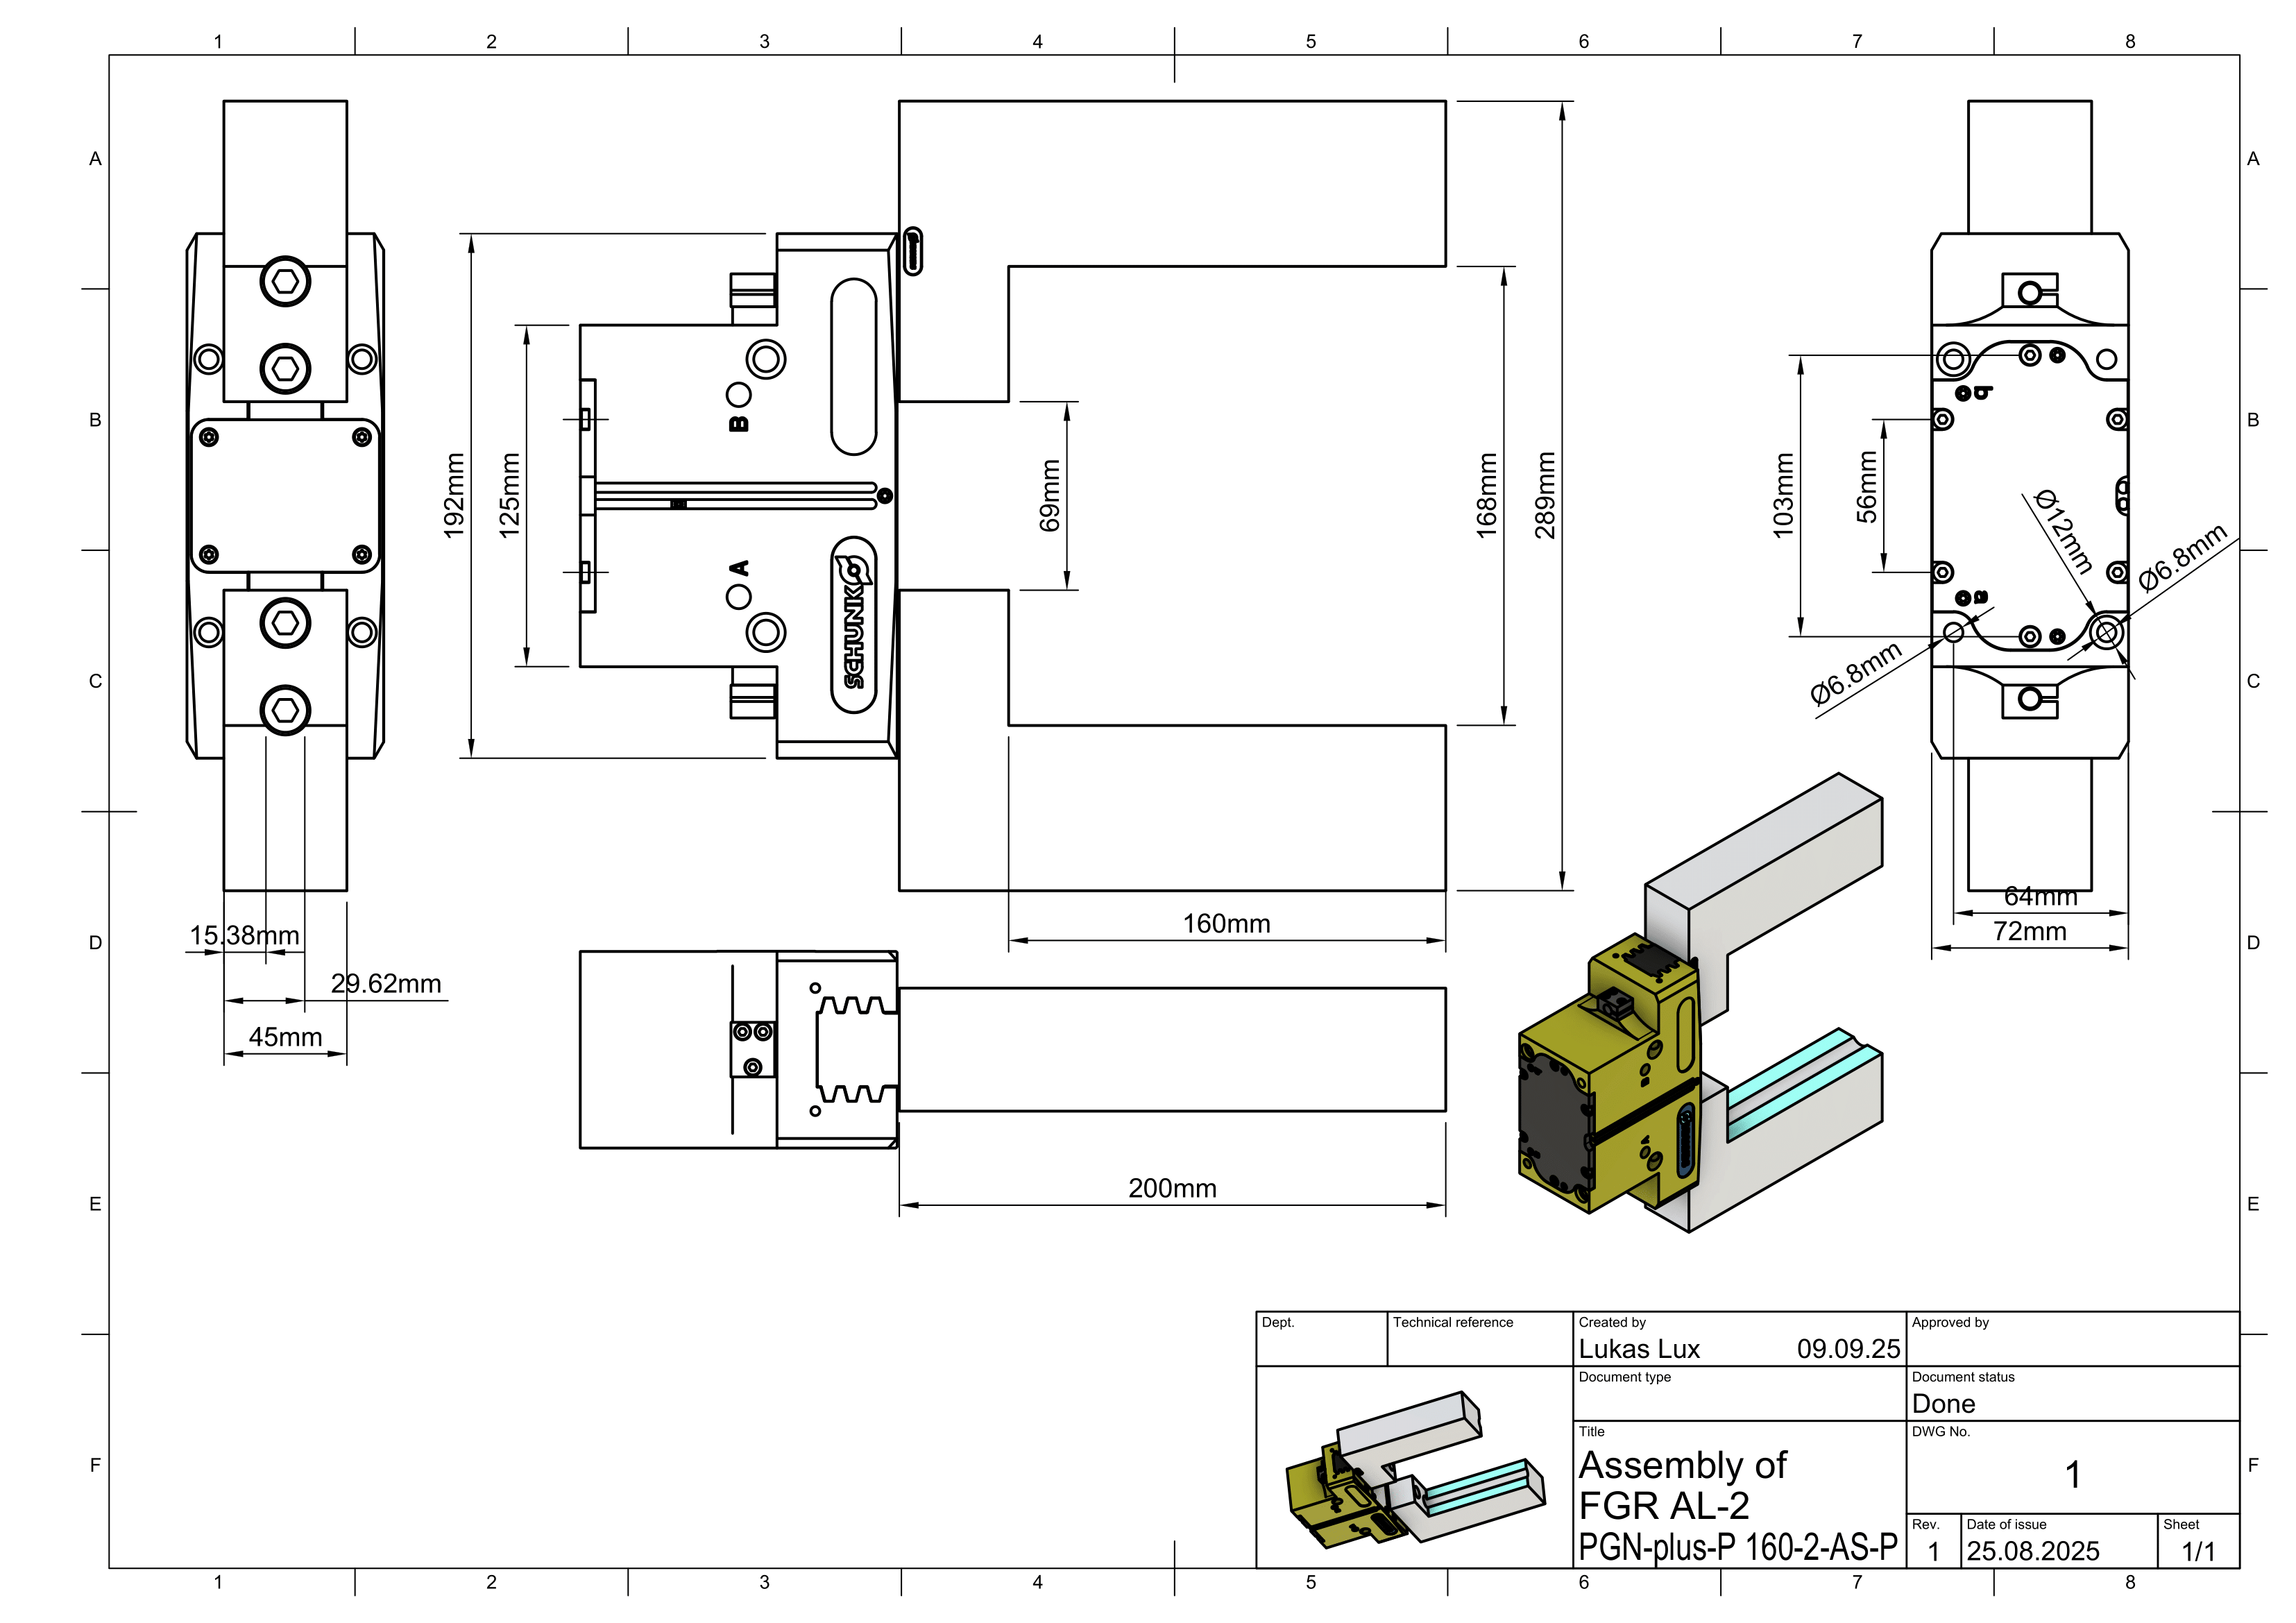
\includegraphics[width=\linewidth]{Figures/SchunkGreifer-1.png}
  \caption{Technische Zeichnung des ausgelegten Parallelgreifers, dargestellt
  mithilfe von Autodesk Fusion 360}
  \label{figure:schunkGripper}
\end{figure}

\subsection{Flange als Visualisierungstool}
Im Rahmen dieses Frameworks wird das Unity-Package \textit{Flange} genutzt.
Implementiert durch GitHub-User \textit{Preliy} und frei verfügbar im Rahmen
einer BSD 3-Clause Lizenz, bietet ein spezialisiertes Framework für die
Robotersteuerung in Unity mit modularer Architektur, die Gelenksteuerung,
Kinematik, Koordinatentransformationen und Echtzeitüberwachung als separate
Komponenten organisiert. Das System unterstützt sowohl direkte
Gelenkmanipulation auf niedriger Ebene als auch kartesische Steuerung auf
höherer Abstraktionsebene, wodurch es für verschiedene Roboteranwendungen
einsetzbar ist.\vglcite{preliyflange2024} Im Kontext dieser Entwicklungsarbeit
wird Flange zur Implementierung und Visualisierung der
Denavit-Hartenberg-Parameter und damit einhergehender Achstransformationen
eingesetzt. Die Notation nach Denavit-Hartenberg ermöglicht als
fundamentales Werkzeug der Robotik eine
systematische Beschreibung der Geometrie serieller Robotermechanismen
und somit die Anwendung etablierter algorithmischer Verfahren für kinematische
Berechnungen, Berechnung von Jacobi-Matrizen sowie
Bewegungsplanung.\vglcite[590]{corke2007}

Flange ermöglicht eine direkte Konfiguration des Roboters über \textit{Frame}
und \textit{JointTransformation} Scripts. Ein Frame definiert dabei die
Denavit-Hartenberg-Parameter für einen Teil der kinematischen Kette, eine
JointTransformation die Parameter des Gelenks, also möglicher
maximaler Ausschlag
in positive und negative Achsrotationsrichtung sowie maximale Geschwindigkeit
und Beschleunigung. Diese Funktion werden im Rahmen dieser Implementierung
genutzt, um den zu simulierenden Roboter theoretisch nachvollziehbar im Raum
bewegen zu können.

\subsection{Modellierung in Unity}
Der Arbeitsraum wurde der vorangegangenen Darstellung entsprechend in Unity
modelliert. Dabei wurden die von Unity standardmäßig gewählten Einstellungen
verwendet, sowohl bei der Modellierung als auch im Kontext der
Physik-Engine. Jegliche Hindernisse wurden dabei mit Collidern versehen und dem
Tag \texttt{Obstacle} und respektive \texttt{Machine} für die Maschine, um diese
bei der späteren Auswertung als Hindernisse kenntlich zu machen. Weiterführend
wurden den einzelnen Stationen (linkes und rechtes Regal, Maschine) das Script
\texttt{Station.cs} angehängt und dort im Sinne des bereits beschriebenen
Arbeitsablaufs ein steigender Index zugewiesen. Analog dazu wird allen
Zylinderkopf-Objekten das Script \texttt{Part.cs} zugewiesen, welche diese als
Werkstücke identifiziert und mit dem durch Drag-and-Drop im Unity Inspector die
Reihenfolge der einzelnen Stationen definiert wird, welche das Teil durchlaufen
muss.

Alle Monitore wurden in einer einheitlichen Unity-Testumgebung ausgeführt.
Die Simulationen basieren auf einem Abbild des Roboters, der
kontinuierlich seine Gelenkwinkel und Zustände an die Monitore übermittelt.
Die erkannten Ereignisse werden unmittelbar protokolliert und in eine
JSON-Logdatei geschrieben. Auf diese Weise sind die Ergebnisse der
verschiedenen Monitore konsistent dokumentiert und in
Kapitel~\ref{cap:Ergebnisse} direkt vergleichbar.


\section{Datenaufzeichnung und Logging}
\label{sec:logging}
Als zentrales Aufzeichnungsformat implementiert der \texttt{SafetyMonitor} eine
JSON-Struktur für die durch die einzelnen Module erzeugten Ereignisse.
Die Key-Value-Paare dieser Objekte sind durch die Klassen
\texttt{RobotStateSnapshot} und \texttt{SafetyEvent} vordefiniert.
Wird ein Ereignis ausgelöst, so wird ein neues \texttt{SafetyEvent} instanziert
(vgl. Abbildung~\ref{listing:SafetyEvent}).

\begin{figure}[H]
  \inputminted[fontsize=\footnotesize]{csharp}{code-snippets/SafetyEvent.cs}
  \caption{SafetyEvent-Klasse mit Zuordnung zum Monitor und Kritikalität}
  \label{listing:SafetyEvent}
\end{figure}

Der \texttt{RobotStateSnapshot} kann initial leer sein, da durch Multithreading
nicht in jedem Fall eine direkte Referenz zum aktuellen Roboterzustand vorliegt.
Über die Methode \texttt{SetEventData()} der \texttt{SafetyEvent}-Klasse werden
anschließend die spezifischen Daten ergänzt, beispielsweise die
Kollisionsposition
bei einer Kollisionserkennung.

Der \texttt{SafetyMonitor} ergänzt das Ereignis um den aktuellen
\texttt{RobotStateSnapshot}, der zusätzliche Informationen wie
aktuelle Achswinkel,
Motordaten, Programmzeiger und Programmname enthält
(vgl. Abbildung~\ref{listing:RobotStateSnapshot}).
Die Events werden zwischengespeichert und am Ende der Ausführung gesammelt
als JSON-Datei in einem vordefinierten Ordner abgelegt.

\begin{figure}[H]
  \inputminted[fontsize=\footnotesize]{csharp}{code-snippets/RobotStateSnapshot.cs}
  \caption{RobotStateSnapshot-Klasse mit formalisieren Attributen}
  \label{listing:RobotStateSnapshot}
\end{figure}

